\documentclass[12pt]{article}

% This first part of the file is called the PREAMBLE. It includes
% customizations and command definitions. The preamble is everything
% between \documentclass and \begin{document}.

\usepackage[margin=1in]{geometry}  % set the margins to 1in on all sides
\usepackage{graphicx}              % to include figures
\usepackage{amsmath}               % great math stuff
\usepackage{amsfonts}              % for blackboard bold, etc
\usepackage{amsthm}                % better theorem environments
\usepackage{amssymb} 
\usepackage{mathptmx}
\usepackage{enumerate}
\usepackage{graphicx}
\usepackage{listings}
\usepackage{xcolor}

% various theorems, numbered by section

\newtheorem{thm}{Theorem}[section]
\newtheorem{lem}[thm]{Lemma}
\newtheorem{prop}[thm]{Proposition}
\newtheorem{cor}[thm]{Corollary}
\newtheorem{conj}[thm]{Conjecture}
\newtheorem{mydef}[thm]{Definition}
\lstset{
	basicstyle          =   \sffamily,          
	keywordstyle        =   \bfseries,          
	commentstyle        =   \rmfamily\itshape,  
	stringstyle         =   \ttfamily,  
	flexiblecolumns,                
	numbers             =   left,   
	showspaces          =   false,  
	numberstyle         =   \fontsize{5}{skip},    
	showstringspaces    =   false,
	captionpos          =   t,      
	frame               =   lrtb,   
}

\lstdefinestyle{cpp}{
	language        =   cpp, 
	basicstyle      =   \fontsize{5}{skip},
	numberstyle     =   \fontsize{5}{skip},
	keywordstyle    =   \color{blue},
	keywordstyle    =   [2] \color{teal},
	stringstyle     =   \color{magenta},
	commentstyle    =   \color{red}\ttfamily,
	breaklines      =   true,   
	columns         =   fixed,  
	basewidth       =   0.5em,
}
\begin{document}


\title{ CSE 120 Spring 2021\\
	Homework Assignment 1}

\author{Jaden Liu \\
	zliu259@ucsc.edu\\ 
University of California at Santa Cruz\\
Santa Cruz, CA 95064 USA }

\maketitle


\section{HW1} 

\textbf{1. Two engineers solve the same problem, but each has a different solution (A and B). Using the default compiler options, the A program takes 6 seconds to run on processor P1 when compiled, and 5 seconds for the B program. This means that B is 1.2 times faster with the default options.
}\\
\begin{enumerate}[a)]
	\item If we enable the gcc optimizations, we increase the CPI by 1.3 times and decrease the
	dynamic instruction count by 20\% for program B (program A remains the same). What is the
	new speedup? (1 point)
	\item If we also enable the compiler optimizations for the A program, we increase CPI by 70\%. How
	much does the instruction count need to change (increase or decrease?) so that it matches the
	performance of both programs (both with optimizations)? (1 point)
\end{enumerate}

\begin{proof}[Solution for a]
	\begin{align*}
		speedup&=\frac{T_{oldA}}{oldB}\cdot\frac{T_{old}}{T_{new}}\\
		&=\frac{T_{oldA}}{oldB}\cdot\frac{Instruction\ count_{old} \cdot CPI_{old} \cdot Clock\ Cycle\ Time_{old}}{Instruction\ count_{new} \cdot CPI_{new} \cdot Clock\ Cycle\ Time_{new}}\\
		&=\frac{6}{5}\cdot\frac{1}{1.3*0.8}\\
		&=\frac{6}{5}\cdot\frac{1}{1.04}\\
		&\approx1.1538
	\end{align*}
\end{proof}

\begin{proof}[Solution for b]
	Assume new instruction count x times the old instruction count.
	\begin{align*}
		speedup_b&=\frac{T_{oldB}}{T_{newB}}\\
		&=\frac{Instruction\ count_{old} \cdot CPI_{old} \cdot Clock\ Cycle\ Time_{old}}{Instruction\ count_{new} \cdot CPI_{new} \cdot Clock\ Cycle\ Time_{new}}\\
		&=\frac{1}{1.7\cdot x} = speedup_a = \frac{1}{1.04}\\
		\text{Solving the equation we get:}\\
		x&=\frac{52}{85}\\
		&\approx0.6117
	\end{align*}
Therefore, instruction count needs to decrease $(1-0.6117)*100\%=38.83$\% so that it matches the
performance of both programs
\end{proof}

\textbf{2. The following table shows how many cycles each type of instruction takes and what the
	percentage in a given P processor}\\
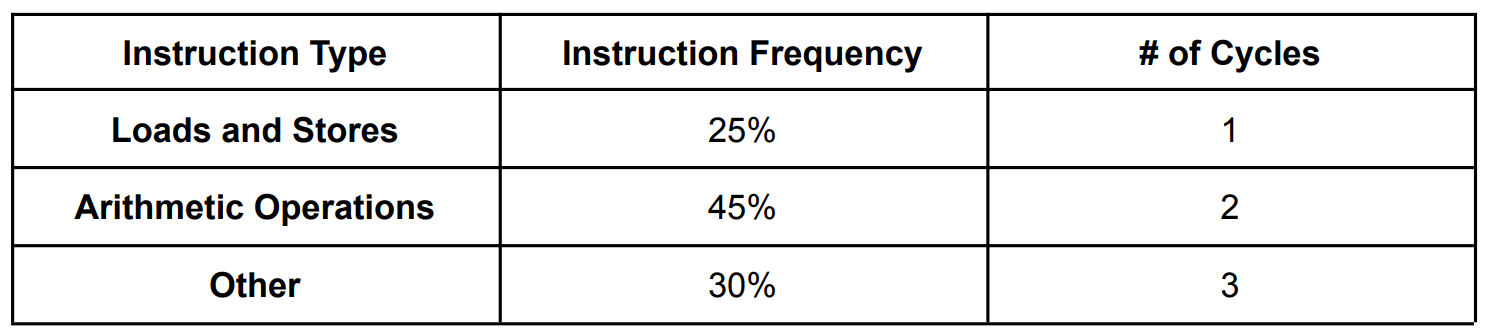
\includegraphics[scale=0.3]{1.png}

\begin{enumerate}[a)]
	\item Given the information in the table above, calculate the CPI and IPC. (1 point)
	\item Now if some engineering effort is done on P to improve the arithmetic operations by
	25\%. Calculate the new CPI? (1 point)
	\item What is the maximum speedup if the loads and stores are optimized? (1 point)
\end{enumerate}

\begin{proof}[Solution for a]
	\begin{align*}
		CPI&=25\%\cdot1+45\%\cdot2+30\%\cdot3\\
		&=0.25+0.9+0.9\\
		&=2.05\\
		IPC&=\frac{1}{CPI}\\
		&=\frac{20}{41}\\
		&\approx0.4878
	\end{align*}
\end{proof}
\begin{proof}[Solution for b]
	\begin{align*}
		CPI&=25\%\cdot1+45\%\cdot2\cdot0.75+30\%\cdot3\\
		&=0.25+0.675+0.9\\
		&=1.825\\
	\end{align*}
\end{proof}

\begin{proof}[Solution for c]
	By Amdahl's law, we can get maximum CPI is $0.25+0.9=1.15$
	\begin{align*}
		speedup&=\frac{T_{old}}{T_{new}}\\
		&=\frac{Instruction\ count_{old} \cdot CPI_{old} \cdot Clock\ Cycle\ Time_{old}}{Instruction\ count_{new} \cdot CPI_{new} \cdot Clock\ Cycle\ Time_{new}}\\
		&=\frac{2.05}{1.15}\\
		&\approx1.7826
	\end{align*}
\end{proof}

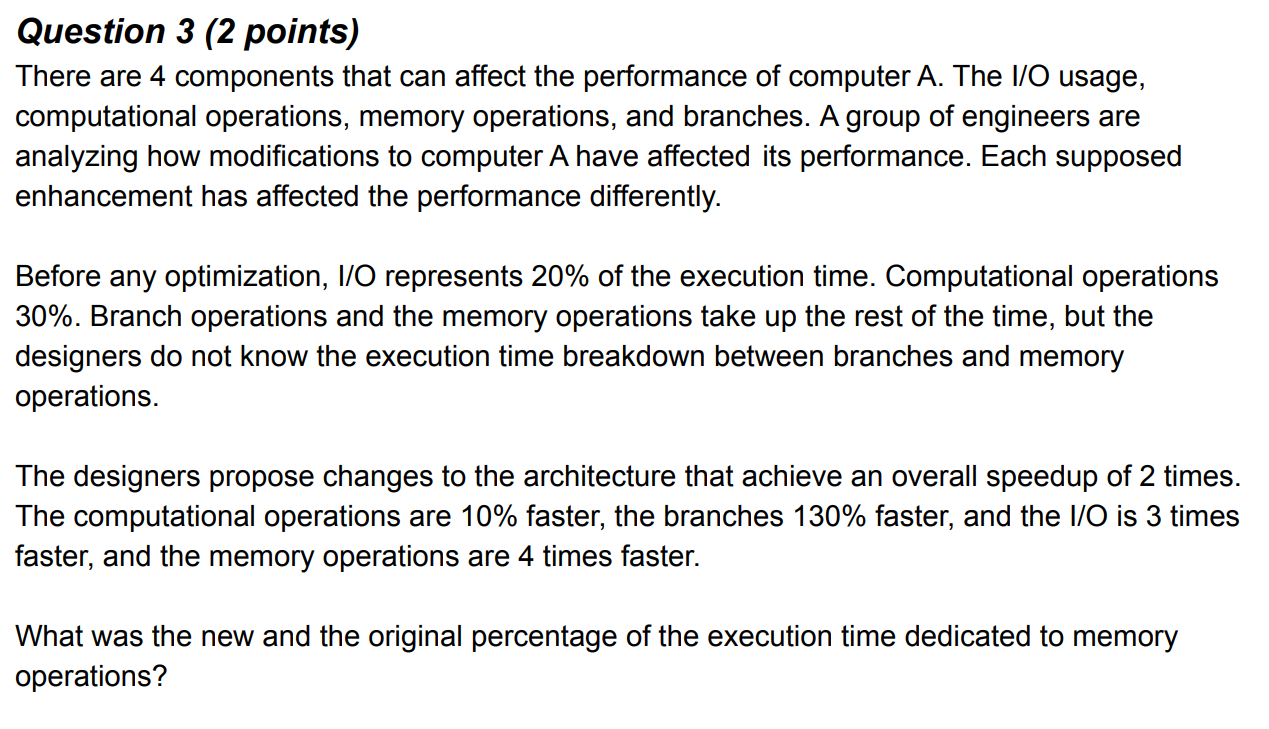
\includegraphics[scale=0.36]{3.png}
\begin{proof}[Solution]
	Let the branches and memory operation execution time be $x$, and $y$, then we have the equations
	\begin{equation}
		\left\{
		\begin{aligned} 
			\frac{0.3}{1.1}+\frac{0.2}{3}+\frac{x}{2.3}+\frac{y}{4}=0.5\\
			x+y=0.5
		\end{aligned}
		\right.
	\end{equation}
	\begin{equation}
	\left\{
	\begin{aligned} 
		x&\approx0.192692\\
		y&\approx0.307308
	\end{aligned}
	\right.
\end{equation}
Thus, the branches take approximately 19.27\% and memory operations take 30.73\% in the total execution time. 
\end{proof}

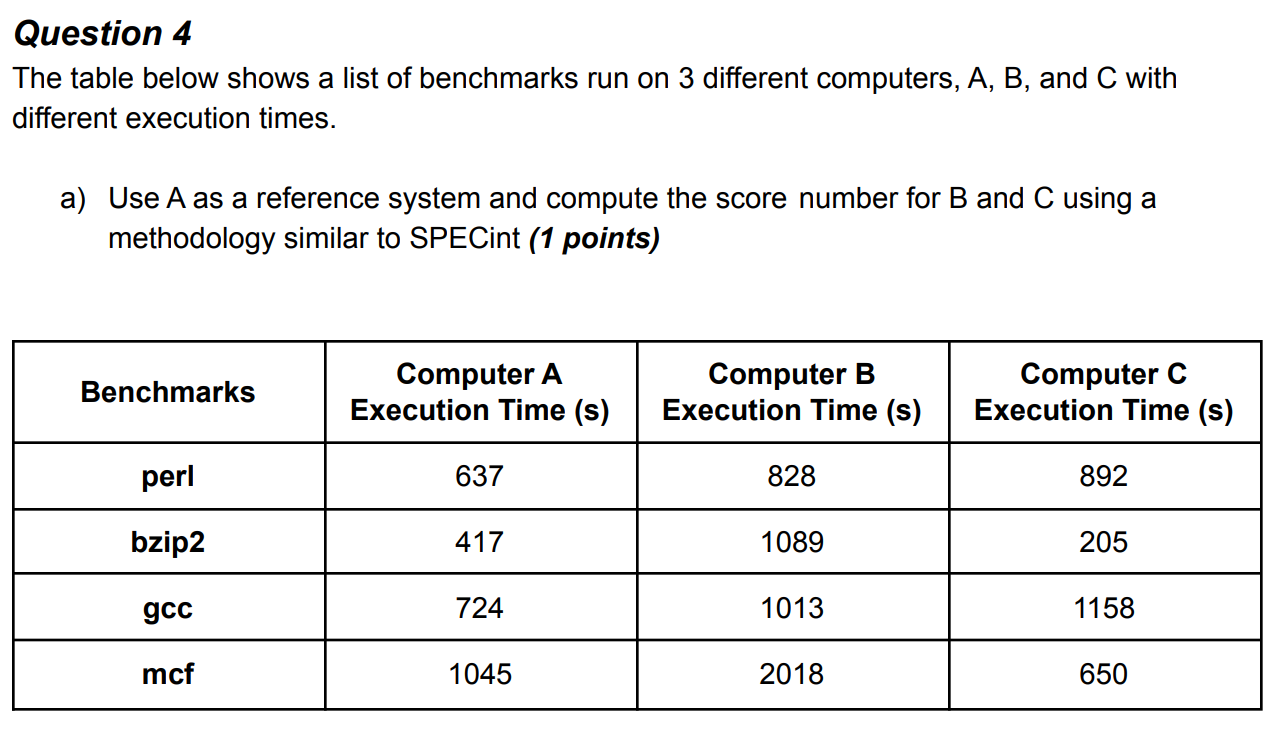
\includegraphics[scale=0.35]{4_1.png}\\
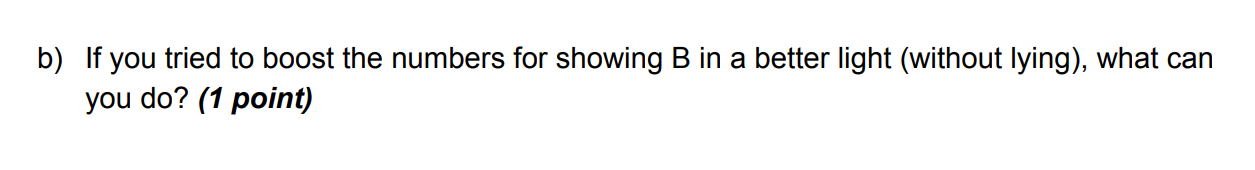
\includegraphics[scale=0.35]{4_2.png}\\
\begin{proof}[Solution for a]
	Using arithmetic mean to compute the speed up based on A\\
	\centering
	\begin{tabular}{lrrr}
		Benchmarks & \multicolumn{1}{l}{ A Execution Time} & \multicolumn{1}{l}{ B Execution Time} & \multicolumn{1}{l}{C Execution Time } \\
		perl  & 1     & 1.2998 & 1.4003 \\
		bzip2 & 1     & 2.6115 & 0.4916 \\
		gcc   & 1     & 1.3992 & 1.5995 \\
		mcf   & 1     & 1.9311 & 0.622 \\
		arithmetic mean & 1     & 1.8104 & 1.02835 \\
		speedup base A & 1     & 0.552364118 & 0.972431565 \\
	\end{tabular}%
\end{proof}

\begin{proof}[Solution for b]
	Using geometric mean to compute the speed up based on A, so we can gain better speed up.\\
	\centering
 	\begin{tabular}{lrrr}
 		Benchmarks & \multicolumn{1}{l}{ A Execution Time} & \multicolumn{1}{l}{ B Execution Time} & \multicolumn{1}{l}{C Execution Time } \\
 		perl  & 1     & 1.2998 & 1.4003 \\
 		bzip2 & 1     & 2.6115 & 0.4916 \\
 		gcc   & 1     & 1.3992 & 1.5995 \\
 		mcf   & 1     & 1.9311 & 0.622 \\
 		geometric mean & 1     & 1.740254561 & 0.909707757 \\
 		speedup base A & 1     & 0.574628576 & 1.09925412 \\
 	\end{tabular}%
\end{proof}

\textbf{5. Iron’s Law helps us calculate the program run time and is the product of instruction per program, clock period, and cycles per instruction.\\Program A is running on the processor P1 with a clock rate of 1.61 GHz. This program consists of 13 billion instructions. Program A has a floating-point multiplication instruction type that is executed 40\% of the time and takes 5 cycles and the remaining instructions take 3 cycles on average to finish.}\\

\begin{enumerate}[a)]
	\item What is the execution time of program A? (1 point)
	\item With some engineering investments, the machine compiler is enhanced to execute more instructions and allows a floating-point multiplication to take place three times as fast and rest of the instructions to finish in half the time. How long does it take program A to finish now? (1 point)
	\item What is the gained speedup? (1 point)
\end{enumerate}
\begin{proof}[Solution for a]
	\begin{align*}
		\text{Time per Program} &= \text{(instruction per program) * CPI * Clock Period}\\
		&=13*10^9\cdot(0.4*5+0.6*3)\cdot\frac{1}{1.61GHZ}\\
		&=30.6832
	\end{align*}
\end{proof}

\begin{proof}[Solution for b]
	\begin{align*}
		\text{Time per Program} &= \text{(instruction per program) * CPI * Clock Period}\\
		&=13*10^9\cdot(0.4*5/3+0.6*3/2)\cdot\frac{1}{1.61GHZ}\\
		&=12.6501
	\end{align*}
\end{proof}
\begin{proof}[Solution for c]
	\begin{align*}
		speedup&=\frac{T_{old}}{T_{new}}\\
		&=\frac{Instruction\ count_{old} \cdot CPI_{old} \cdot Clock\ Cycle\ Time_{old}}{Instruction\ count_{new} \cdot CPI_{new} \cdot Clock\ Cycle\ Time_{new}}\\
		&=\frac{30.6832}{12.6501}\\
		&=2.42553
	\end{align*}
\end{proof}
\textbf{6. You need to write the following expression in 4 different ISAs using the high-level assembly used in class: $d = (b+a)*(b*a)+a$
}\\

\begin{enumerate}[a)]
	\item For a generic accumulator-based architecture (1 point)
	\item For a generic Register-Memory Architecture (1 point)
	\item  For a generic Load-Store Architecture (1 point)
	\item For a RISC-V ISA (1 point)
\end{enumerate}
\begin{proof}[Solution for a]
	\begin{lstlisting}[language={python},numbers=left,numberstyle=\tiny,%frame=shadowbox,  
	rulesepcolor=\color{red!20!green!20!blue!20},  
	keywordstyle=\color{blue!70!black},  
	commentstyle=\color{blue!90!},  
	basicstyle=\ttfamily]  
	
	ld(a)
	add b
	mult b
	mult a
	add a
	st (d)
\end{lstlisting}
\end{proof}

\begin{proof}[Solution for b]
	\begin{lstlisting}[language={python},numbers=left,numberstyle=\tiny,%frame=shadowbox,  
		rulesepcolor=\color{red!20!green!20!blue!20},  
		keywordstyle=\color{blue!70!black},  
		commentstyle=\color{blue!90!},  
		basicstyle=\ttfamily]  
		
	ld,R1,(b)
	add,R2,R1,(a)
	mult,R3,R1,(a)
	add,R4,R2,R3
	st,R4,(d)
	\end{lstlisting}
\end{proof}

\begin{proof}[Solution for c]
	\begin{lstlisting}[language={python},numbers=left,numberstyle=\tiny,%frame=shadowbox,  
		rulesepcolor=\color{red!20!green!20!blue!20},  
		keywordstyle=\color{blue!70!black},  
		commentstyle=\color{blue!90!},  
		basicstyle=\ttfamily]  
		
	ld,R1,(b)
	ld,R2,(a)
	add,R3,R1,R2
	mult,R4,r1,r2
	add,R5,R3,R4
	st,R5,(d)
	\end{lstlisting}
\end{proof}
\begin{proof}[Solution for d]
	\begin{lstlisting}[language={python},numbers=left,numberstyle=\tiny,%frame=shadowbox,  
		rulesepcolor=\color{red!20!green!20!blue!20},  
		keywordstyle=\color{blue!70!black},  
		commentstyle=\color{blue!90!},  
		basicstyle=\ttfamily]  
		
	lw r1,0(b)
	lw r2,0(a)
	add r3,r1,r2
	mult r4,r1,r2
	add r5,r3,r4
	sw r5,0(d)
	\end{lstlisting}
\end{proof}
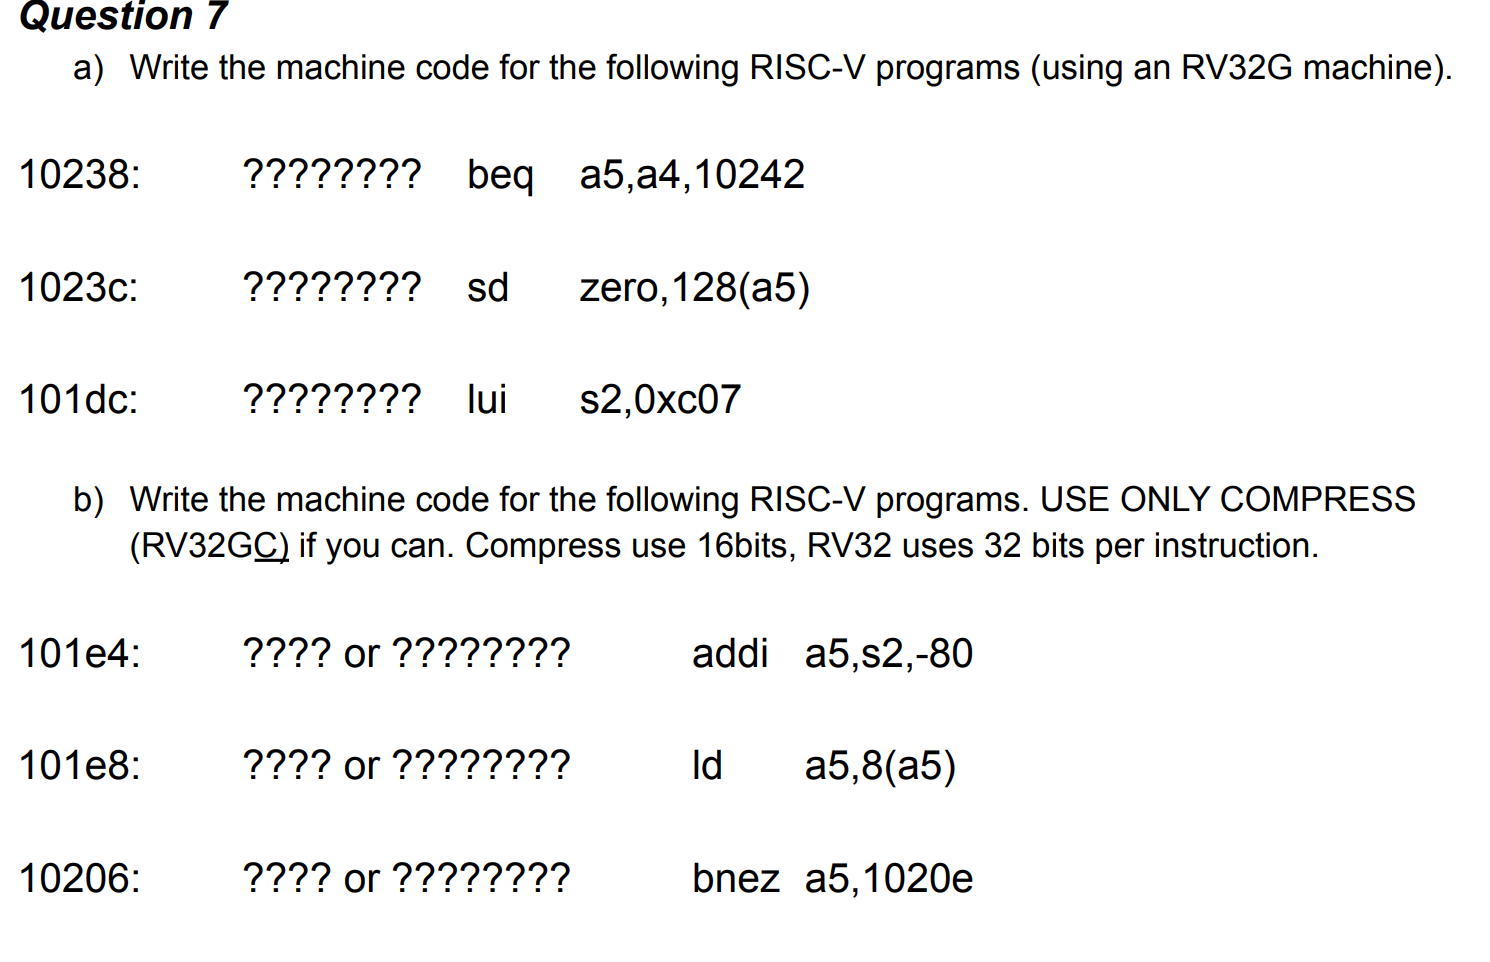
\includegraphics[scale=0.3]{7.png}
\begin{proof}[Solution for a]
	\ \\
	\begin{enumerate}
		\item 0x10242-0x10238=0xa=0b0000 0000 1010\\
		0b0 000000 01110 01111 000 0101 0 1100011\\
		\textbf{0x00E78563}
		\item 0d128:0b10000000\\
		0b0000100 00000 01111 010 00000 0100011\\
		\textbf{0x0807A023}
		\item 0b00000000110000000111 10010 0110111\\
		\textbf{0x00C07937}
	\end{enumerate}
\end{proof}

\begin{proof}[Solution for b]
	\ \\
	\begin{enumerate}
		\item 0d-80:0b111110110000\\
		0b111110110000 10010 000 01111 0010011\\
		\textbf{RV32G:0xFB090793}\\
		can't express in RV32C
		\item 0d8:1000\\
		ob000000001000 01111 010 01111 0000011\\
		\textbf{RV32G:0x0087A783}\\
		0b 010 010 111 0 0 111 00\\
		\textbf{RV32C:0x4B9C}
		\item 0x1020e-0x10206=0x8=0b 0000 0000 1000\\
		0b 0000000 00000 01111 001 10000 1100011\\
		\textbf{RV32G:0x00079863}\\
		0b111 0 10 111 00 00 0 01\\
		\textbf{RV32C:0xEB81}
	\end{enumerate}
\end{proof}
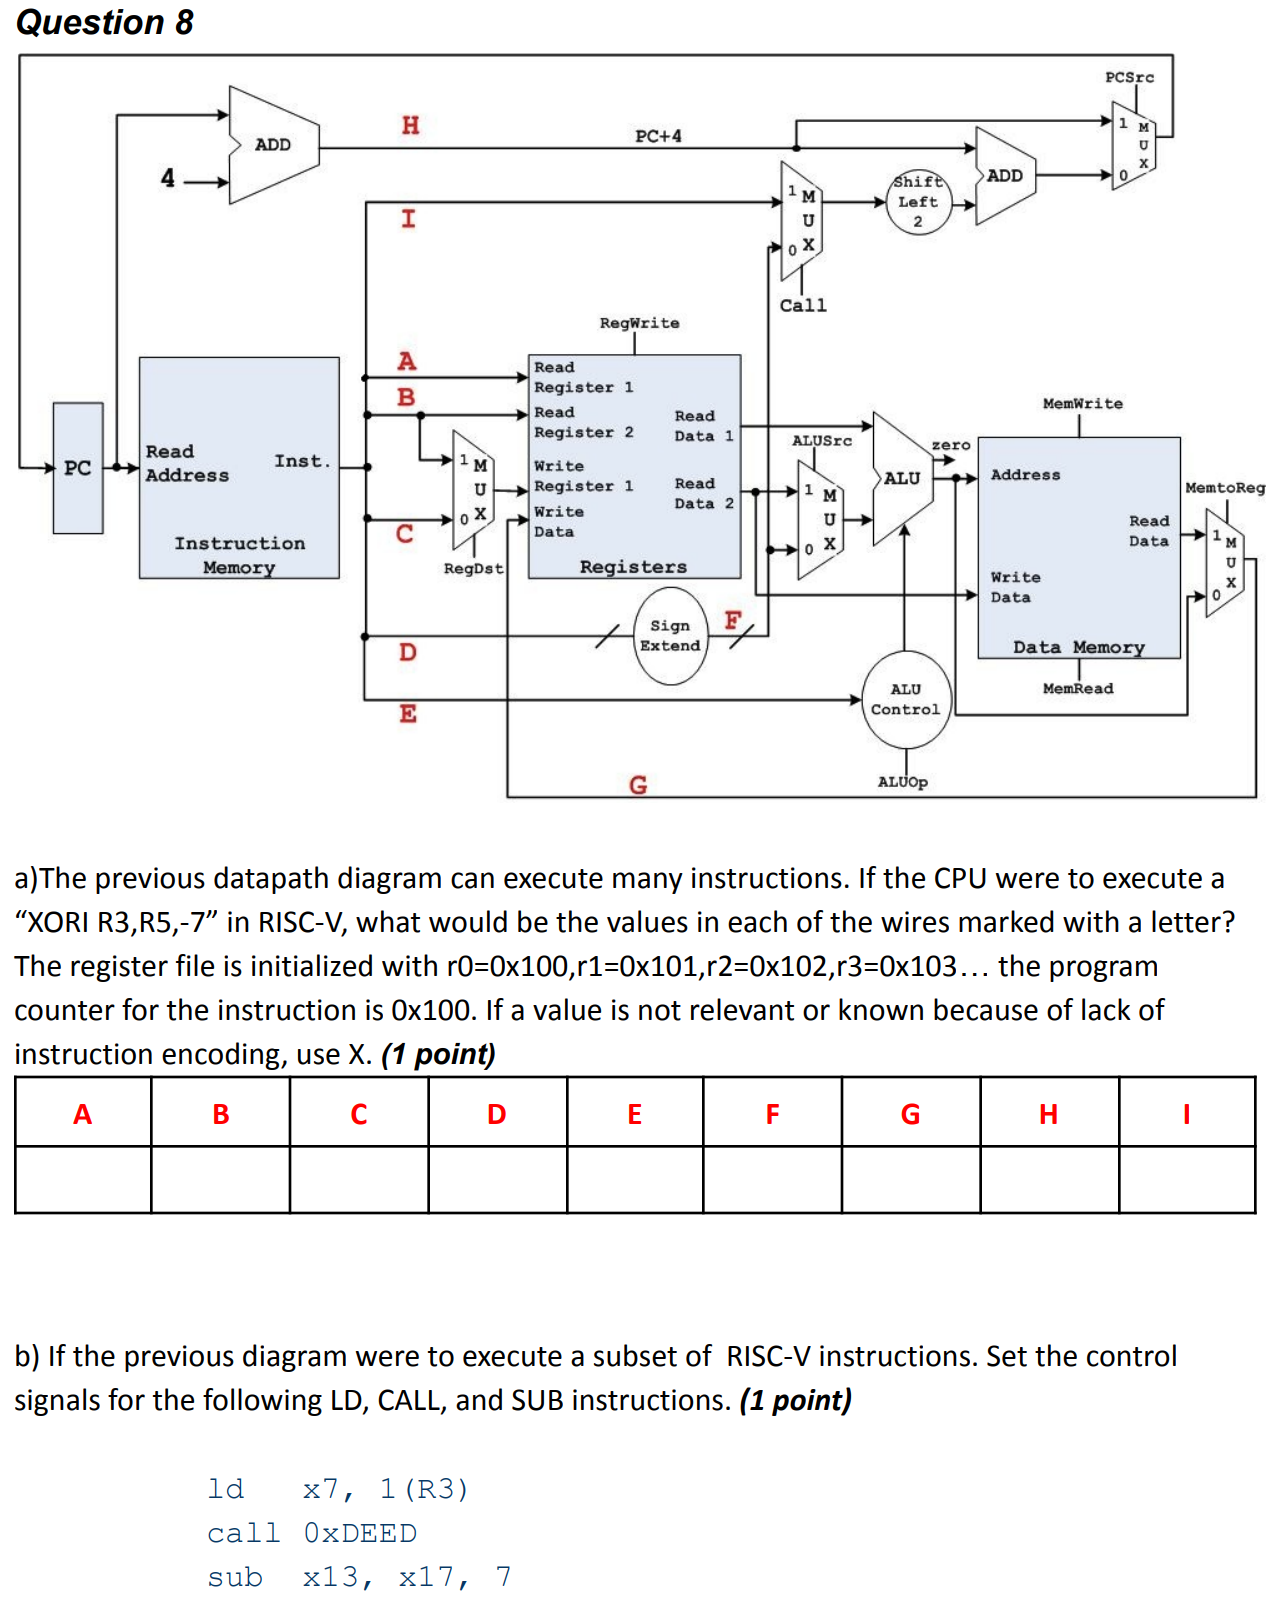
\includegraphics[scale=0.35]{8.png}
\begin{proof}[Solution for a]
	\centering
	\begin{tabular}{lllllllll}
		a     & b     & c     & d     & e     & f     & g     & h     & i \\
		R5 & X     & R3 & -7  & XORI   & sign extend -7 & f xor 0x105 & 0x104 & X \\
	\end{tabular}%
\end{proof}
\begin{proof}[Solution for b]
	\ \\
	\centering
	    \begin{tabular}{llrrlrrrr}
		& BR    & \multicolumn{1}{l}{JP} & \multicolumn{1}{l}{ALUsrc} & ALUop & \multicolumn{1}{l}{Dmwe} & \multicolumn{1}{l}{Rwe} & \multicolumn{1}{l}{Rdst} & \multicolumn{1}{l}{Rwd} \\
		lw x7, 1(r3) & X     & 0     & 0     & lw    & 0     & 1     & 0     & 1 \\
		call 0xDEED (auipc) & X     & 0     & 0     & auipc & 0     & 1     & 0     & 1 \\
		call 0xDEED (jalr) & X     & 1     & 0     & jalr  & 0     & 1     & 0     & 1 \\
		sub x13,x17,7 & X     & 0     & 1     & sub   & 0     & 1     & 0     & 1 \\
	\end{tabular}%

\end{proof}

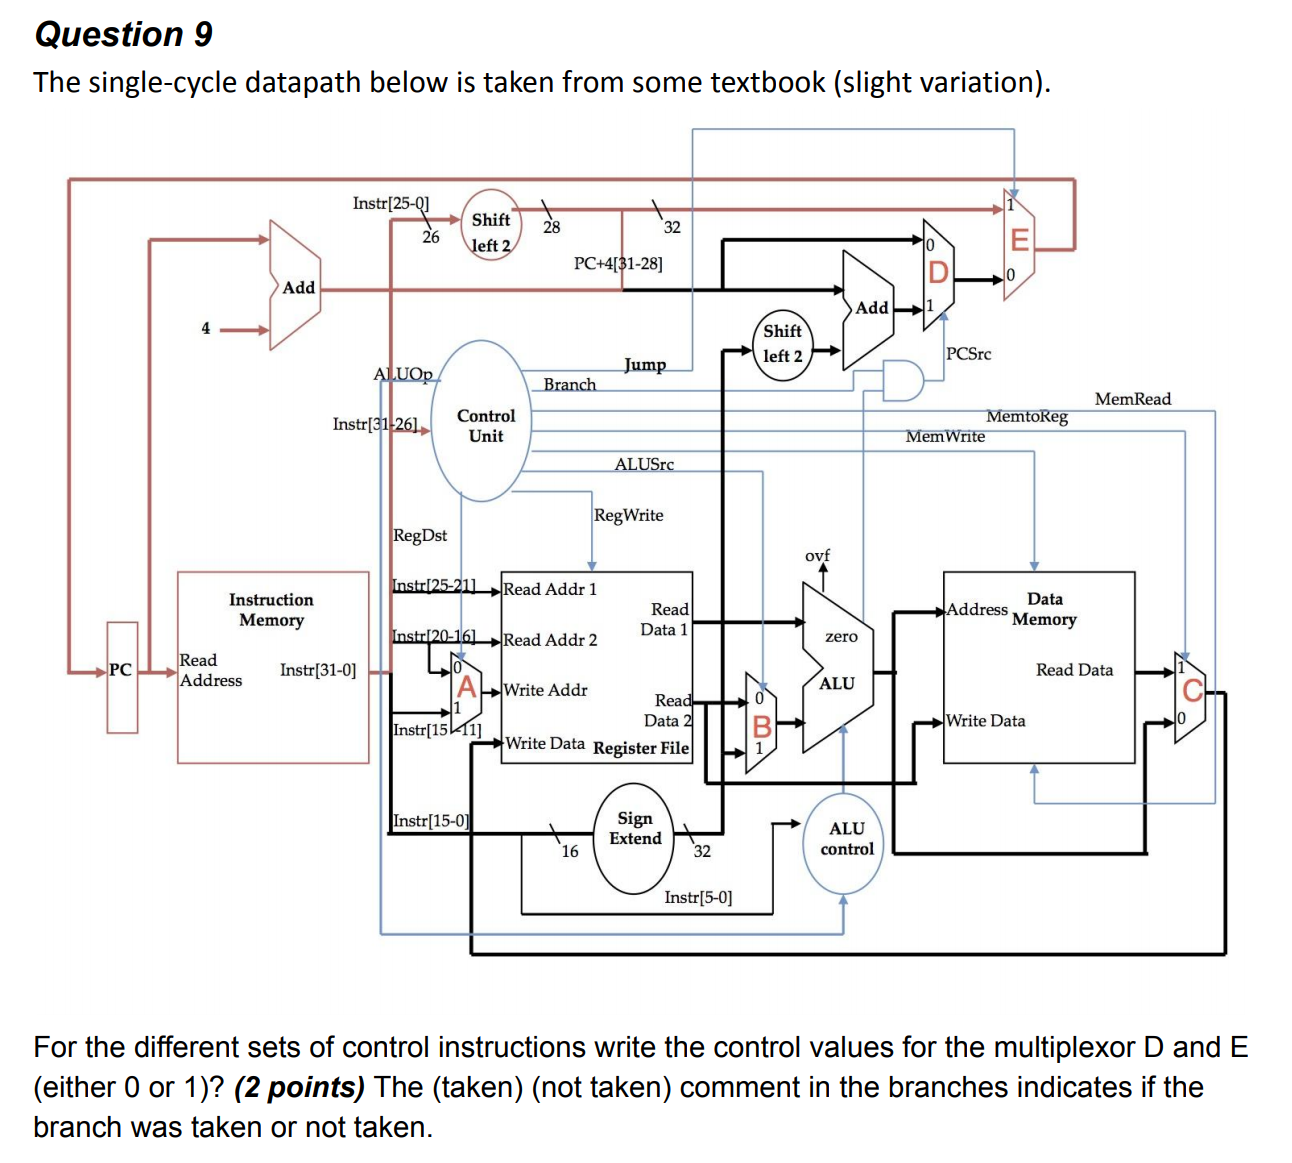
\includegraphics[scale=0.35]{9.png}
\begin{proof}[Solution]
	\centering
	\begin{tabular}{lrr}
		Instruction & \multicolumn{1}{l}{MUX D} & \multicolumn{1}{l}{MUX E} \\
		jr x30 & X     & 1 \\
		bne x1,x0,foo(not taken) & 0     & 0 \\
		jalr x0, 0xFF00 & X      & 1 \\
		ret   & X     & 1 \\
		jal 0xAAC0 & X     & 1 \\
		beq x1,x0,bar(taken) & 1     & 0 \\
	\end{tabular}%
\end{proof}
\bigskip



\end{document}
